% DOCUMENT CLASS SETUP
\documentclass[12pt, a4paper]{article}

% DOCUMENT PACKAGES
\usepackage[a4paper, margin=1in]{geometry}
\usepackage{titling}
\usepackage{enumitem}
\usepackage{amsmath}
\usepackage{amssymb}
\usepackage{mathtools}
\usepackage{graphicx}
\usepackage{xcolor}
\usepackage{listings}
\usepackage{hyperref}
\usepackage{csquotes}

% FONT AND ENCODING SETUP
\usepackage{fontspec}
\usepackage{polyglossia}
\usepackage[Thai]{ucharclasses}
\setdefaultlanguage{english}
\setotherlanguage{thai}
\setTransitionsFor{Thai}{\thaifont}{\normalfont}
\newfontfamily{\thaifont}{THSarabun.ttf}[
    Path=./,
    BoldFont=THSarabunBold.ttf,
    ItalicFont=THSarabunItalic.ttf,
    BoldItalicFont=THSarabunBoldItalic.ttf,
    Scale=1.23
]
\XeTeXlinebreaklocale "th"
\XeTeXlinebreakskip = 0pt plus 1pt

% PROFESSIONAL CODE BLOCK
\usepackage{tcolorbox}
\tcbuselibrary{minted, skins, breakable}

% DEFINE GITHUB DARK THEME COLORS %
\definecolor{ghback}{HTML}{0d1117}    % Dark background
\definecolor{ghtext}{HTML}{c9d1d9}    % Light gray text
\definecolor{ghborder}{HTML}{30363d}  % GitHub Border color

% PROFESSIONAL CODE BLOCK CONFIGURATION (MINTED VERSION) %
\renewcommand{\theFancyVerbLine}{\textcolor{white!60!gray}{\scriptsize\arabic{FancyVerbLine}}}
\newtcblisting{codeblock}[2][]{
    enhanced,
    breakable,
    colback=ghback,
    colframe=ghborder,
    coltitle=ghtext,
    colupper=ghtext,
    fonttitle=\bfseries\small,
    arc=3mm,
    boxrule=0.5mm,
    % PADDING SETTINGS
    left=25pt,
    right=10pt,
    top=5pt,
    bottom=5pt,
    % MINTED SETTINGS
    listing engine=minted,
    listing only,
    minted language=python,
    minted options={
        linenos,
        numbersep=5pt,
        fontsize=\footnotesize,
        breaklines=true,
        breakanywhere=true,
        autogobble,
        style=monokai,
    },
    title={#2},
    #1
}

% DOCUMENT TITLE SETUP %
\title {
	\textbf{2110573 PATTERN RECOGNITION} \\
    \vspace{1em}
	\Large{\textbf{Homework 5: PyTorch \& Transformer}} \\
    \vspace{0.5em}
    \large{Computer Engineering, Chulalongkorn Univerity}
}
\author{Worralop Srichainont}
\date{\today}
\setlength{\droptitle}{15em}

% DOCUMENT CONTENTS
\begin{document}

    \maketitle
    \thispagestyle{empty}
    \clearpage

    \tableofcontents
    \thispagestyle{empty}
    \clearpage

    \pagenumbering{arabic}

    \part{Precipitation Nowcasting}
        Precipitation nowcasting is the the task of predicting the amount of rainfall
        in a certain region given some kind of sensor data.
        The term nowcasting refers to tasks that try to predict the current or near future conditions
        (within 6 hours).

        \vspace{0.5em}

        You will be given satellite images in 3 different bands covering a 5 by 5 region from different parts of Thailand.
        In other words, your input will be a $5 \times 5 \times 3$ image.
        Your task is to predict the amount of rainfall in the center pixel.
        You will first do the prediction using just a simple fully-connected neural network that view each pixel as different input features.

        \vspace{0.5em}

        Since the your input is basically an image, we will then view the input as an image and apply CNN to do the prediction.
        Finally, we can also add a time component since weather prediction can benefit greatly using previous time frames.
        Each data point actually contain 5 time steps, so each input data point has a size of $5 \times 5 \times 5 \times 3$
        (time $\times$ height $\times$ width $\times$ channel), and the output data has a size of 5 (time).
        You will use this time information when you work with RNNs.

        \vspace{0.5em}

        Finally, we would like to thank the Thai Meteorological Department for providing the data for this assignment.

        \vspace{1em}

        \textbf{Please access the Kaggle Notebook here:} \texttt{\url{https://www.kaggle.com/code/worralopsrichainont/2110573-patt-recog-hw5}}

    \pagebreak

        \section{Problem T1}
            Explain each line of code in the function \texttt{preprocess\_for\_ff()}
            \begin{codeblock}{Problem T1}
                def preprocess_for_ff(x_train, y_train, x_val, y_val):
                    x_train_ff = x_train.reshape((-1, 5 * 5 * 3))
                    y_train_ff = y_train.reshape((-1, 1))
                    x_val_ff = x_val.reshape((-1, 5 * 5 * 3))
                    y_val_ff = y_val.reshape((-1, 1))
                    x_test_ff = x_test.reshape((-1, 5 * 5 * 3))
                    y_test_ff = y_test.reshape((-1, 1))

                    return x_train_ff, y_train_ff, x_val_ff, y_val_ff, x_test_ff, y_test_ff
            \end{codeblock}

            \vspace{1em}

            \noindent \underline{\textbf{Answer}}

            \begin{enumerate}
                \item The original image are $5 \times 5$ pixels with RGB colors channel.
                \item Flatten each $5 \times 5 \times 3$ image from \texttt{x\_train} to a 1D array of 75 numbers.
                \item Reshape the training labels (\texttt{y\_train}) to a \texttt{sample\_size} $\times 1$ 2D array.
                \item Repeat the step 2-3 for validation dataset (\texttt{x\_val} and \texttt{y\_val})
                and test dataset (\texttt{x\_test} and \texttt{y\_test})
                \item Return the preprocessed data
            \end{enumerate}

        \section{Problem T2}
            Why is the loss MSE?

            \begin{codeblock}{Problem T2}
                loss_fn = nn.MSELoss()
            \end{codeblock}

            \vspace{1em}

            \noindent \underline{\textbf{Ans.}} The model is trying to predict the amount of rainfall at a given time step
            and the rainfall is the continuous numerical value. Therefore, it is the regression task and MSE loss is suitable for it.

	\pagebreak

        \section{Problem T3}
            Below, the code for creating a 3-layers fully connected neural network in PyTorch is provided.
            Run the code and make sure you understand what you are doing.
            Then, report the results.

            \begin{codeblock}{Problem T3}
                class FeedForwardNN(nn.Module):
                    def __init__(self, hidden_size=200):
                        super(FeedForwardNN, self).__init__()
                        self.ff1 = nn.Linear(75, hidden_size)
                        self.ff2 = nn.Linear(hidden_size, hidden_size)
                        self.ff3 = nn.Linear(hidden_size, hidden_size)
                        self.out = nn.Linear(hidden_size, 1)

                    def forward(self, x):
                        hd1 = F.relu(self.ff1(x))
                        hd2 = F.relu(self.ff2(hd1))
                        y = F.relu(self.ff3(hd2))
                        y = self.out(y)
                        return y.reshape(-1, 1)
            \end{codeblock}

            \noindent \underline{\textbf{Answer}}

            \begin{itemize}
                \item The final dense layer has no activation function as can be seen in \texttt{y = self.out(y)}.
                \item \textbf{ReLU} would actually be a better activation function for the final dense layer,
                because the rainfall cannot be negative and ReLU can ensure that every prediction are not negative rainfall value.
            \end{itemize}

	\pagebreak

        \section{Problem T4}
            Explain why the first linear layer has number of parameters equals to 15200?

            \begin{table}[h]
                \centering
                \begin{tabular}{|c|c|c|}
                    \hline
                    \textbf{Layer} & \textbf{Output Shape} & \textbf{Parameters} \\
                    \hline \hline
                    FeedForwardNN & [1024, 1] & - \\
                    Linear: 1-1 & [1024, 200] & 15,200 \\
                    Linear: 1-2 & [1024, 200] & 40,200 \\
                    Linear: 1-3 & [1024, 200] & 40,200 \\
                    Linear: 1-4 & [1024, 1] & 201 \\
                    \hline
                \end{tabular}
                \caption{Model Summary}
            \end{table}
            
            \vspace{1em}

            \noindent \underline{\textbf{Answer}}

            \vspace{0.25em}

            \noindent According to the following \texttt{FeedForwardNN} model code.

            \begin{codeblock}{Problem T4}
                class FeedForwardNN(nn.Module):
                    def __init__(self, hidden_size=200):
                        super(FeedForwardNN, self).__init__()
                        self.ff1 = nn.Linear(75, hidden_size)
                        # MORE LAYERS...
            \end{codeblock}

            \noindent The code shows that the layer \texttt{ff1} has 75 input nodes and 200 output nodes
            \begin{itemize}
                \item \textbf{Weight}: $75 \times 200 = 15,000$ parameters
                \item \textbf{Bias}: 200 parameters
                \item \textbf{Total}: 15,000 + 200 = 15,200 parameters
            \end{itemize}
        
    \pagebreak

        \section{Problem T5}
            Plot \texttt{loss} and \texttt{val\_loss} as a function of epochs.

            \vspace{1em}

            \noindent \underline{\textbf{Answer}}

            \vspace{0.25em}

            \noindent Use this following \texttt{matplotlib} code to plot the loss of each epoch.
            \begin{codeblock}{Problem T5}
                # Generate a sequence of epoch numbers for the x-axis
                epochs = range(1, len(train_losses) + 1)

                # Create the plot
                plt.figure(figsize=(10, 6))
                plt.plot(epochs, train_losses, 'b-', label='Training Loss (MSE)')
                plt.plot(epochs, val_losses, 'r-', label='Validation Loss (MSE)')

                # Add labels, title, and legend
                plt.title('Training and Validation Losses over Epochs')
                plt.xlabel('Epoch')
                plt.ylabel('Loss (MSE)')
                plt.legend()
                plt.grid(True)

                # Display the plot
                plt.show()
            \end{codeblock}

            \noindent The result shows as follows
            \begin{figure}[h]
                \centering
                
\includegraphics[width=0.6\textwidth]{image_01}
                \caption{Fully Connected Model Loss}
            \end{figure}

        \section{Problem T6}
            When does the model starts to overfit?

            \vspace{1em}

            \noindent \underline{\textbf{Ans.}} According to the graph in the problem T5,
            the model starts to overfit around epoch 2 or 3, because it starts to get better
            at predicting the training data starts getting worse at predicting validation data.

    \pagebreak

        \section{Problem T7}
            Plot the learning rate as a function of the epochs.

            \vspace{1em}

            \noindent \underline{\textbf{Answer}}

            \vspace{0.25em}

            \noindent Use this following \texttt{matplotlib} code to plot the learning rate of each epoch.
            \begin{codeblock}{Problem T7}
                # Generate a sequence of epoch numbers for the x-axis
                epochs = range(1, len(learning_rates) + 1)

                # Create the plot
                plt.figure(figsize=(10, 6))
                plt.plot(epochs, learning_rates, 'g-o', label='Learning Rate', linewidth=2, markersize=6)

                # Add labels, title, and legend
                plt.title('Learning Rate over Epochs')
                plt.xlabel('Epoch')
                plt.ylabel('Learning Rate')
                plt.legend()
                plt.grid(True)

                # Display the plot
                plt.show()
            \end{codeblock}

            \noindent The result shows as follows
            \begin{figure}[h]
                \centering
                
\includegraphics[width=0.6\textwidth]{image_02}
                \caption{Fully Connected Model Learning Rate}
            \end{figure}

        \section{Problem T8}
            What makes the learning rate change?

            \vspace{1em}

            \noindent \underline{\textbf{Ans.}} The learning rates changes because of the ReduceLROnPlateau
            scheduler. It monitors the validation loss and check if the validation loss stop getting lower
            for 2 epoch. If the model stop improving for 2 epochs, it reduces learning rate.

    \pagebreak

    \part{Scheduler \& Evaluation}

        \noindent Use the code snippet below to load the model you just trained in the previous part

        \begin{codeblock}{Load Model}
            checkpoint = torch.load("model_ff.pth.tar")
            loaded_model = FeedForwardNN(hidden_size=config["hidden_size"])  # Create model object
            loaded_model.load_state_dict(checkpoint["model"])  # Load weights
            print(f"Loaded epoch {checkpoint['epoch']} model")
        \end{codeblock}

        \section{Problem T9}
            The scheduler can be very complicated and you can write your own heuristic for it.
            Implement a custom learning rate scheduler that behaves like the following graph.

            \begin{figure}[h]
                \centering
                
\includegraphics[width=0.5\textwidth]{image_03}
            \end{figure}

            \subsection{Implementation}
                \begin{codeblock}{Problem T9 - Implementation}
                    class MyScheduler:
                        def __init__(self, optimizer: torch.optim.Optimizer):
                            self.optimizer = optimizer
                            self.base_lrs = [group['lr'] for group in optimizer.param_groups]

                        def step(self, epoch):
                            scale_factor = 0.8 ** epoch

                            # Apply the new learning rate to the optimizer
                            for i, group in enumerate(self.optimizer.param_groups):
                                new_lr = self.base_lrs[i] * scale_factor
                                group['lr'] = new_lr
                \end{codeblock}

    \pagebreak

            \subsection{Training}

                \begin{codeblock}{Problem T9 - Initialization}
                    # Initialize model and optimizer
                    model_ff = FeedForwardNN(hidden_size=config["hidden_size"]).to(device)
                    optimizer = torch.optim.Adam(model_ff.parameters(), lr=config["lr"])

                    # Initialize scheduler
                    my_scheduler = MyScheduler(optimizer)

                    # Track performance
                    train_losses = []
                    val_losses = []
                    learning_rates = []
                \end{codeblock}

                \begin{codeblock}{Problem T9 - Training}
                    for epoch in range(config["epochs"]):
                        # Training
                        train_loss = []
                        current_lr = optimizer.param_groups[0]["lr"]
                        learning_rates.append(current_lr)

                        # Flag model as training.
                        model_ff.train()

                        print(f"Training epoch {epoch+1}...")
                        print(f"Current LR: {current_lr}")

                        for i, (inputs, y_true) in enumerate(tqdm(train_loader)):
                            # Transfer data from cpu to gpu
                            inputs = inputs.to(device)
                            y_true = y_true.to(device)

                            # Reset the gradient
                            optimizer.zero_grad()

                            # Predict
                            y_pred = model_ff(inputs)

                            # Calculate loss
                            loss = loss_fn(y_pred, y_true)

                            # Compute gradient
                            loss.backward()

                            # Update parameters
                            optimizer.step()

                            # Log stuff
                            train_loss.append(loss)

                        avg_train_loss = torch.stack(train_loss).mean().item()
                        train_losses.append(avg_train_loss)

                        print(f"Epoch {epoch+1} train loss: {avg_train_loss:.4f}")

                        # Validation
                        model_ff.eval()
                        with torch.no_grad():  # No gradient is required during validation
                            print(f"Validating epoch {epoch+1}")
                            val_loss = []
                            for i, (inputs, y_true) in enumerate(tqdm(val_loader)):
                                # Transfer data from cpu to gpu
                                inputs = inputs.to(device)
                                y_true = y_true.to(device)

                                # Predict
                                y_pred = model_ff(inputs)

                                # Calculate loss
                                loss = loss_fn(y_pred, y_true)

                                # Log stuff
                                val_loss.append(loss)

                            avg_val_loss = torch.stack(val_loss).mean().item()
                            val_losses.append(avg_val_loss)
                            print(f"Epoch {epoch+1} val loss: {avg_val_loss:.4f}")

                        # Update the learning rate at the end of the epoch
                        my_scheduler.step(epoch + 1)
                \end{codeblock}

    \pagebreak

        \section{Problem T10}
            Write a function to evaluate your model.
            Your function must predicts using the input model
            and return mean square error of the model.

            \vspace{1em}

            \noindent \underline{\textbf{Answer}}

            \vspace{0.25em}

            \begin{codeblock}{Problem T10}
                def evaluate(data_loader, model):
                    """
                    Evaluate model on validation data given by data_loader
                    """
                    # Set the model to evaluation mode
                    model.eval()

                    # Initialize MSE loss function
                    loss_fn = nn.MSELoss()

                    # Safely get the device the model is currently on
                    device = next(model.parameters()).device

                    batch_losses = []

                    # Disable gradient calculation to save memory and speed up inference
                    with torch.no_grad():
                        for inputs, y_true in data_loader:
                            # Transfer data to the correct device (GPU/CPU)
                            inputs = inputs.to(device)
                            y_true = y_true.to(device)
                            
                            # Forward pass: make predictions
                            y_pred = model(inputs)
                            
                            # Calculate MSE loss for this batch
                            loss = loss_fn(y_pred, y_true)
                            batch_losses.append(loss)

                    # Calculate the mean of all batch losses and convert to a standard Python float
                    mse = torch.stack(batch_losses).mean().item()

                    return mse
            \end{codeblock}

            \noindent The evaluation compared to the baseline (majority rule) are this follows:
            \begin{table}[h]
                \centering
                \begin{tabular}{|c|c|c|}
                    \hline
                    \textbf{Source} & \textbf{Train MSE} & \textbf{Validation MSE} \\
                    \hline \hline
                    Majority Baseline & 1.944 & 1.675 \\
                    Fully Connected Model & 1.918 & 1.656 \\
                    \hline
                \end{tabular}
                \caption{Fully Connected Model Evaluation}
            \end{table}

	\pagebreak

        \section{Problem T11}
            You might notice that the 3-layered feedforward does not use dropout at all.
            Now, try adding dropout (dropout rate of 20\%) to the model, run, and report the result again.

            \vspace{0.5em}

            \noindent In this problem, write a feedforward model with dropout.

			\vspace{1em}

            \noindent \underline{\textbf{Answer}}

            \vspace{0.25em}

            \begin{codeblock}{Problem T11}
                class FeedForwardNNDropout(nn.Module):
                    def __init__(self, hidden_size=200, dropout_rate=0.5):
                        super(FeedForwardNNDropout, self).__init__()
                        # Linear layers
                        self.ff1 = nn.Linear(75, hidden_size)
                        self.ff2 = nn.Linear(hidden_size, hidden_size)
                        self.ff3 = nn.Linear(hidden_size, hidden_size)
                        self.out = nn.Linear(hidden_size, 1)
                        
                        # Dropout layer
                        # p is the probability of an element to be zeroed out
                        self.dropout = nn.Dropout(p=dropout_rate)

                    def forward(self, x):
                        # Apply dropout after the ReLU activation for each hidden layer
                        hd1 = self.dropout(F.relu(self.ff1(x)))
                        hd2 = self.dropout(F.relu(self.ff2(hd1)))
                        y = self.dropout(F.relu(self.ff3(hd2)))
                        
                        # Output layer (no dropout applied here)
                        y = self.out(y)
                        return y.reshape(-1, 1)
            \end{codeblock}

	\pagebreak

        \section{Problem T12}
            \noindent Please complete the code to train your dropout model.

            \vspace{1em}

            \noindent \underline{\textbf{Answer}}

            \vspace{0.25em}

            \begin{codeblock}{Problem T12 - Initialization}
                # Initialize the new dropout model
                model_ff_dropout = FeedForwardNNDropout(hidden_size=config["hidden_size"], dropout_rate=0.5)
                model_ff_dropout = model_ff_dropout.to(device)

                # Initialize the optimizer and scheduler
                optimizer = torch.optim.Adam(model_ff_dropout.parameters(), lr=config["lr"])
                scheduler = torch.optim.lr_scheduler.ReduceLROnPlateau(
                    optimizer, "min", 
                    factor=config["scheduler_factor"],
                    patience=config["scheduler_patience"],
                    min_lr=config["scheduler_min_lr"]
                )

                # Lists to keep track of losses
                train_losses_dropout = []
                val_losses_dropout = []
            \end{codeblock}
			See training codeblock in the next page $\rightarrow$

	\pagebreak

            \begin{codeblock}{Problem T12 - Training}
                for epoch in range(config["epochs"]):
                    # TRAINING
                    model_ff_dropout.train()
                    train_loss = []
                    
                    current_lr = optimizer.param_groups[0]["lr"]
                    print(f"\nTraining epoch {epoch+1} (LR: {current_lr})...")
                    
                    for inputs, y_true in tqdm(train_loader):
                        inputs = inputs.to(device)
                        y_true = y_true.to(device)
                        
                        optimizer.zero_grad()
                        y_pred = model_ff_dropout(inputs)
                        loss = loss_fn(y_pred, y_true)
                        loss.backward()
                        optimizer.step()
                        
                        train_loss.append(loss.detach())
                        
                    avg_train_loss = torch.stack(train_loss).mean().item()
                    train_losses_dropout.append(avg_train_loss)

                    # VALIDATION
                    model_ff_dropout.eval()
                    val_loss = []
                    
                    with torch.no_grad():
                        for inputs, y_true in tqdm(val_loader):
                            inputs = inputs.to(device)
                            y_true = y_true.to(device)
                            
                            y_pred = model_ff_dropout(inputs)
                            loss = loss_fn(y_pred, y_true)
                            val_loss.append(loss.detach())
                            
                    avg_val_loss = torch.stack(val_loss).mean().item()
                    val_losses_dropout.append(avg_val_loss)

                    print(f"Epoch {epoch+1} | Train Loss: {avg_train_loss:.4f} | Val Loss: {avg_val_loss:.4f}")

                    # Step the scheduler based on the validation loss
                    scheduler.step(avg_val_loss)
            \end{codeblock}

\pagebreak

        \section{Problem T13}
            Plot the losses and MSE of the training and validation as before.
            Evaluate the dropout model's performance

            \subsection{Plotting}
                \noindent Use this following \texttt{matplotlib} code to plot the loss of each epoch.

                \begin{codeblock}{Problem T13 - Plotting}
                    # Plot here
                    # Generate the x-axis values based on the number of epochs recorded
                    epochs_dropout = range(1, len(train_losses_dropout) + 1)

                    # Create the plot
                    plt.figure(figsize=(10, 6))
                    plt.plot(epochs_dropout, train_losses_dropout, 'b-', label='Training Loss (Dropout)')
                    plt.plot(epochs_dropout, val_losses_dropout, 'r-', label='Validation Loss (Dropout)')

                    # Add labels, title, and legend
                    plt.title('Training vs Validation Loss with Dropout')
                    plt.xlabel('Epoch')
                    plt.ylabel('Loss (MSE)')
                    plt.legend()
                    plt.grid(True)

                    # Display the plot
                    plt.show()
                \end{codeblock}

                \noindent The result shows as follows
                \begin{figure}[h]
                    \centering
                    
\includegraphics[width=0.8\textwidth]{image_04}
                    \caption{Fully Connected with Dropout Model Loss}
                \end{figure}

	\pagebreak

            \subsection{Evaluation}
                \begin{codeblock}{Problem T13 - Evaluation}
                    passdropout_mse = evaluate(val_loader, model_ff_dropout)
                    print(f"Dropout Model Validation MSE: {dropout_mse:.4f}")
                \end{codeblock}

                \noindent The evaluation compared to the baseline (majority rule) are this follows:
                \begin{table}[h]
                    \centering
                    \begin{tabular}{|c|c|c|}
                        \hline
                        \textbf{Source} & \textbf{Train MSE} & \textbf{Validation MSE} \\
                        \hline \hline
                        Majority Baseline & 1.944 & 1.675 \\
                        Fully Connected Model & 1.918 & 1.656 \\
                        Fully Connected Model (Dropout) & 1.923 & 1.661 \\
                        \hline
                    \end{tabular}
                    \caption{Fully Connected Model with Dropout Evaluation}
                \end{table}

    \pagebreak

    \part{Convolutional Neural Networks}
        Now let's try to incorporate the grid structure to your model.
        Instead of passing in vectors, we are going to pass in the $5 \times 5$ grid into the model.
        You are going to implement you own 2D Convolutional Neural Networks (CNN) with the following structure.

        \begin{table}[h]
            \centering
            \begin{tabular}{|c|c|c|}
                \hline
                \textbf{Layer} & \textbf{Output Shape} & \textbf{Parameters} \\
                \hline \hline
                Conv2DNN & - & - \\
                Conv2d: 1-1 & [1024, 200, 3, 3] & 5,600 \\
                Linear: 1-2 & [1024, 200] & 360,200 \\
                Linear: 1-3 & [1024, 200] & 40,200 \\
                Linear: 1-4 & [1024, 1] & 201 \\
                \hline
            \end{tabular}
            \caption{CNN Model Summary}
        \end{table}

        \section{Problem T14}
            \noindent Please complete the code for preparing data for training CNN.

            \vspace{1em}

            \noindent \underline{\textbf{Answer}}

            \vspace{0.25em}

            \begin{codeblock}{Problem T14 - Functions}
                def get_tensor_x_data_cnn(x_data):
                    x_data_cnn = x_data[:, -1, :, :, :]
                    tensor_x_data_cnn = torch.tensor(x_data_cnn, dtype=torch.float32)
                    tensor_x_data_cnn = tensor_x_data_cnn.permute(0, 3, 1, 2)

                    return tensor_x_data_cnn

                def get_tensor_y_data_cnn(y_data):
                    tensor_y_data_cnn = torch.tensor(y_data, dtype=torch.float32)
                    if len(tensor_y_data_cnn.shape) > 1 and tensor_y_data_cnn.shape[1] > 1:
                        tensor_y_data_cnn = tensor_y_data_cnn[:, -1].unsqueeze(1)
                    
                    return tensor_y_data_cnn
            \end{codeblock}
			See the \texttt{DataLoader} code block in the next page $\rightarrow$

	\pagebreak

            \begin{codeblock}{Problem T14 - DataLoader}
                # Arrange data
                tensor_x_train_cnn = get_tensor_x_data_cnn(x_train)
                tensor_y_train = get_tensor_y_data_cnn(y_train)

                tensor_x_val_cnn = get_tensor_x_data_cnn(x_val)
                tensor_y_val = get_tensor_y_data_cnn(y_val)

                tensor_x_test_cnn = get_tensor_x_data_cnn(x_test)
                tensor_y_test = get_tensor_y_data_cnn(y_val)

                # Create PyTorch Datasets
                train_dataset_cnn = TensorDataset(tensor_x_train_cnn, tensor_y_train)
                val_dataset_cnn = TensorDataset(tensor_x_val_cnn, tensor_y_val)
                test_dataset_cnn = TensorDataset(tensor_x_test_cnn, tensor_y_test)

                # Create PyTorch DataLoaders
                batch_size = 64

                train_loader_cnn = DataLoader(train_dataset_cnn, batch_size=batch_size, shuffle=True)
                val_loader_cnn = DataLoader(val_dataset_cnn, batch_size=batch_size, shuffle=False)
                test_loader_cnn = DataLoader(test_dataset_cnn, batch_size=batch_size, shuffle=False)
            \end{codeblock}

	\pagebreak

        \section{Problem T15}
            \noindent Write a PyTorch Convolutional Neural Network (CNN) model.

            \vspace{1em}

            \noindent \underline{\textbf{Answer}}

            \vspace{0.25em}

            \begin{codeblock}{Problem T15}
                class CNNModel(nn.Module):
                    def __init__(self):
                        super(CNNModel, self).__init__()

                        self.conv1 = nn.Conv2d(in_channels=3, out_channels=16, kernel_size=3, padding=1)
                        self.conv2 = nn.Conv2d(in_channels=16, out_channels=32, kernel_size=3, padding=1)
                        self.pool = nn.MaxPool2d(kernel_size=2, stride=2)

                        self.fc1 = nn.Linear(32 * 1 * 1, 128)
                        self.fc2 = nn.Linear(128, 1)

                    def forward(self, x):
                        # Convolutional layers with ReLU and Pooling
                        x = self.pool(F.relu(self.conv1(x)))
                        x = self.pool(F.relu(self.conv2(x)))

                        # Flatten the feature maps into a 1D vector
                        x = torch.flatten(x, 1) 

                        # Fully connected layers
                        x = F.relu(self.fc1(x))
                        x = self.fc2(x)
                        return x
            \end{codeblock}

	\pagebreak

        \section{Problem T16}
            \noindent Please complete the code to train your CNN model

            \subsection{Model Training}
                \begin{codeblock}{Problem T16 - Initialization}
                    # Initialize the model
                    model_cnn = CNNModel()
                    model_cnn.to(device)

                    # Define Loss function and Optimizer
                    criterion = nn.MSELoss() 
                    optimizer = optim.Adam(model_cnn.parameters(), lr=0.001)

                    # Training Loop
                    num_epochs = 10

                    # Storing losses
                    train_losses = []
                    val_losses = []
                \end{codeblock}

                \begin{codeblock}{Problem T16 - Training}
                    for epoch in range(num_epochs):
                        model_cnn.train() # Set model to training mode
                        running_loss = 0.0
                        
                        # Store losses for the current batch
                        batch_train_losses = [] 
                        
                        for i, data in enumerate(train_loader_cnn, 0):
                            inputs, labels = data
                            
                            # Move data to GPU if available
                            inputs, labels = inputs.to(device), labels.to(device)
                            
                            # Zero the parameter gradients
                            optimizer.zero_grad()

                            # Forward pass
                            outputs = model_cnn(inputs)

                            # Extract only the target for the last timestep
                            if len(labels.shape) > 1 and labels.shape[1] > 1:
                                labels = labels[:, -1].unsqueeze(1)

                            # Ensure labels have the same shape as outputs for MSELoss
                            labels = labels.view_as(outputs)
                            
                            loss = criterion(outputs, labels)
                            
                            # Backward pass and optimize
                            loss.backward()
                            optimizer.step()

                            batch_train_losses.append(loss.item())

                        # Average loss for the epoch
                        epoch_train_loss = sum(batch_train_losses) / len(batch_train_losses)
                        train_losses.append(epoch_train_loss)
                        
                        # Evaluate on validation set after each epoch
                        epoch_val_loss = evaluate(val_loader_cnn, model_cnn)
                        val_losses.append(epoch_val_loss)
                        
                        print(f"Epoch {epoch+1}/{num_epochs} - Train MSE: {epoch_train_loss:.4f}, Val MSE: {epoch_val_loss:.4f}")
                \end{codeblock}
            
            \subsection{Plotting}
                \begin{codeblock}{Problem T16 - Plotting}
                    plt.figure(figsize=(10, 5))
                    plt.plot(train_losses, label='Training Loss')
                    plt.plot(val_losses, label='Validation Loss')
                    plt.title('CNN Model Loss (MSE) Over Epochs')
                    plt.xlabel('Epochs')
                    plt.ylabel('Mean Squared Error')
                    plt.legend()
                    plt.grid(True)
                    plt.show()
                \end{codeblock}

                \noindent The result shows as follows
                \begin{figure}[h]
                    \centering
                    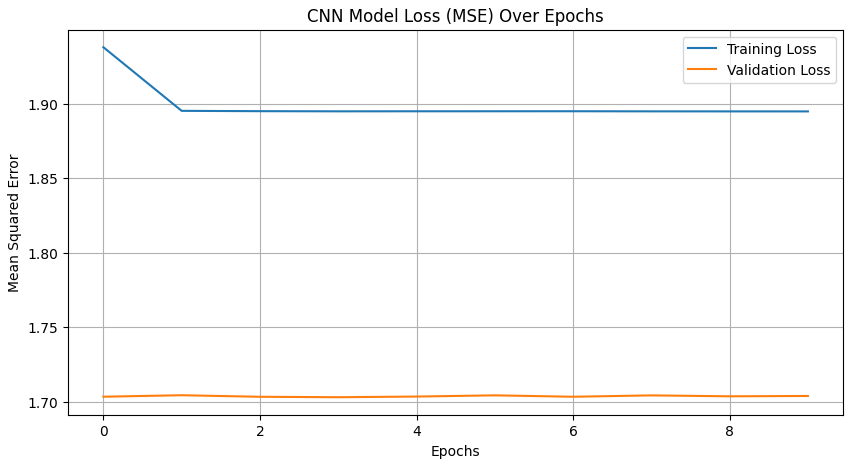
\includegraphics[width=\textwidth]{image_05}
                    \caption{CNN Model Loss}
                \end{figure}

            \subsection{Evaluation}
                \begin{codeblock}{Problem T16 - Evaluation}
                    train_mse = evaluate(train_loader_cnn, model_cnn)
                    val_mse = evaluate(val_loader_cnn, model_cnn)

                    print(f"Final Training MSE: {train_mse:.4f}")
                    print(f"Final Validation MSE: {val_mse:.4f}")
                \end{codeblock}

                \noindent The evaluation compared to the baseline (majority rule) are this follows:
                \begin{table}[h]
                    \centering
                    \begin{tabular}{|c|c|c|}
                        \hline
                        \textbf{Source} & \textbf{Train MSE} & \textbf{Validation MSE} \\
                        \hline \hline
                        Majority Baseline & 1.944 & 1.675 \\
                        Fully Connected Model & 1.918 & 1.656 \\
                        Fully Connected Model (Dropout) & 1.923 & 1.661 \\
                        CNN Model & 1.895 & 1.704 \\
                        \hline
                    \end{tabular}
                    \caption{CNN Model Evaluation}
                \end{table}

    \pagebreak

    \part{Transformer}
        The above models are not usually used in practice due to its limited capability.
        Transformers are generally used by computer vision, natural language processing, and speech processing.

        \begin{table}[h]
            \centering
            \begin{tabular}{|c|c|c|}
                \hline
                \textbf{Layer} & \textbf{Output Shape} & \textbf{Parameters} \\
                \hline \hline
                TransformerModel & [1024, 1] & - \\
                PositionalEncoding: 1-1 & [1024, 5, 76] & - \\
                Dropout: 2-1 & [1024, 5, 76] & - \\
                SelfAttention: 1-2 & [1024, 5, 76] & - \\
                Linear: 2-2 & [1024, 5, 76] & 5,852 \\
                Linear: 2-3 & [1024, 5, 76] & 5,852 \\
                Linear: 2-4 & [1024, 5, 76] & 5,852 \\
                Softmax: 2-5 & [1024, 5, 5] & - \\
                LayerNorm: 1-3 & [1024, 5, 76] & 760 \\
                Linear: 1-4 & [1024, 5, 76] & 5,582 \\
                LayerNorm: 1-5 & [1024, 5, 76] & 760 \\
                Linear: 1-6 & [1024, 1] & 381 \\
                \hline
            \end{tabular}
            \caption{Transformer Model Summary}
        \end{table}

    \pagebreak

        \section{Problem T17}
            In our dataloader, we will add the output of this timestep (the number of precipitation) as an auxiliary input to predict the next timestep.
            \begin{itemize}
                \item \textbf{Input size}: [\texttt{batch\_size}, 5, 76]
                \item \textbf{Output size}: [texttt{batch\_size}, 1]
            \end{itemize}
            Additionally, we will mask the input at the dataloader to the attention from observing future values.
            Suppose that we want to predict timestep 3, we will mask the timestep 3, 4 and 5 in our input by setting it to zeros,
            and we will predict the timestep 3.

            \vspace{0.5em}

            \noindent Please complete the code for preparing data for training Transformer

            \subsection{Dataset Class}
                \begin{codeblock}{Problem T17 - Dataset Class}
                    class TransformerDataset(Dataset):
                        def __init__(self, X, y):
                            # Convert to PyTorch tensors
                            self.X = torch.tensor(X, dtype=torch.float32) if not isinstance(X, torch.Tensor) else X.clone().detach()
                            self.y = torch.tensor(y, dtype=torch.float32) if not isinstance(y, torch.Tensor) else y.clone().detach()

                            self.num_samples = self.X.shape[0]
                            self.seq_len = self.X.shape[1]

                        def __len__(self):
                            return self.num_samples * self.seq_len

                        def __getitem__(self, idx):
                            # Determine which original sample and which timestep to predict
                            sample_idx = idx // self.seq_len
                            t = idx % self.seq_len 

                            # Extract the sequence and ensure targets are 1D
                            X_seq = self.X[sample_idx].clone() # Shape: (5, 75)
                            y_seq = self.y[sample_idx].clone().view(-1) # Shape: (5,)

                            # Add the output of the previous timestep as an auxiliary input
                            # Shift targets by 1
                            y_shifted = torch.zeros(self.seq_len, 1)
                            y_shifted[1:] = y_seq[:-1].unsqueeze(1)
                            
                            # Concatenate features and auxiliary input to get (5, 76)
                            X_combined = torch.cat((X_seq, y_shifted), dim=1) 
                            
                            # Mask current and future timesteps
                            # Suppose we want to predict t = 2, we mask t = 2,3,4 to zeros.
                            X_combined[t:, :] = 0.0
                            
                            # The target is the actual precipitation at timestep t
                            target = y_seq[t].unsqueeze(0) # Shape: (1,)

                            return X_combined, target
                \end{codeblock}

\pagebreak

            \subsection{Create DataLoader}
                \begin{codeblock}{Problem T17 - DataLoader}
                    # Reshape the input data to 3 dimensions: (entries, time-step, features)
                    # Flattening the spatial and channel dimensions into a single feature dimension
                    x_train_trans = x_train.reshape(x_train.shape[0], x_train.shape[1], -1)
                    x_val_trans = x_val.reshape(x_val.shape[0], x_val.shape[1], -1)
                    x_test_trans = x_test.reshape(x_test.shape[0], x_test.shape[1], -1)

                    # Create the custom datasets using your exact 'y' variable names
                    train_dataset_trans = TransformerDataset(x_train_trans, y_train)
                    val_dataset_trans = TransformerDataset(x_val_trans, y_val)
                    test_dataset_trans = TransformerDataset(x_test_trans, y_test)

                    # Create DataLoaders
                    batch_size = 1024

                    train_loader_trans = DataLoader(train_dataset_trans, batch_size=batch_size, shuffle=True)
                    val_loader_trans = DataLoader(val_dataset_trans, batch_size=batch_size, shuffle=False)
                    test_loader_trans = DataLoader(test_dataset_trans, batch_size=batch_size, shuffle=False)
                \end{codeblock}

    \pagebreak

        \section{Problem T18}
            Please write a PyTorch \texttt{PositionalEncoding} Layer.

            \begin{codeblock}{Problem T18}
                class PositionalEncoding(nn.Module):
                    def __init__(self, seq_len, emb_dim, dropout=0.2):
                        super(PositionalEncoding, self).__init__()
                        self.dropout = nn.Dropout(p=dropout)

                        # Create a matrix of shape (seq_len, emb_dim) to hold positional encodings
                        pe = torch.zeros(seq_len, emb_dim)
                        
                        # Create a vector of positions (0, 1, 2, ..., seq_len-1)
                        position = torch.arange(0, seq_len, dtype=torch.float).unsqueeze(1)
                        
                        # Calculate the division term for the sine and cosine arguments
                        div_term = torch.exp(torch.arange(0, emb_dim, 2).float() * (-math.log(10000.0) / emb_dim))
                        
                        # Apply sine to even indices
                        pe[:, 0::2] = torch.sin(position * div_term)
                        
                        # Apply cosine to odd indices
                        pe[:, 1::2] = torch.cos(position * div_term)
                        
                        # Add a batch dimension: (1, seq_len, emb_dim)
                        pe = pe.unsqueeze(0)
                        
                        # Register pe as a buffer (it's not a trainable parameter, but stays with the model)
                        self.register_buffer('pe', pe)

                    def forward(self, x):
                        """
                        Args:
                            x: Input tensor of shape (batch_size, seq_len, emb_dim)
                        """
                        # Add the positional encoding to the input embedding
                        x = x + self.pe[:, :x.size(1), :]
                        return self.dropout(x)
            \end{codeblock}

    \pagebreak

        \section{Problem T19}
            Please write a PyTorch Transformer model.

            \subsection{Self Attention Class}
                \begin{codeblock}{Problem T19 - Self Attention Class}
                    class SelfAttention(nn.Module):
                        def __init__(self, input_dim):
                            super(SelfAttention, self).__init__()
                            # Query, Key, and Value linear transformations
                            self.q = nn.Linear(input_dim, input_dim)
                            self.k = nn.Linear(input_dim, input_dim)
                            self.v = nn.Linear(input_dim, input_dim)
                            self.softmax = nn.Softmax(dim=-1)

                        def forward(self, x):
                            # x shape: (batch_size, seq_len, input_dim)
                            Q = self.q(x)
                            K = self.k(x)
                            V = self.v(x)

                            # Attention scores
                            attention_scores = torch.matmul(Q, K.transpose(-2, -1)) / math.sqrt(x.size(-1))
                            attention_weights = self.softmax(attention_scores)
                            
                            # Weighted sum
                            out = torch.matmul(attention_weights, V)
                            return out
                \end{codeblock}
            
	\pagebreak

            \subsection{Transformer Model}
                \begin{codeblock}{Problem T19 - Transformer Model}
                    class TransformerModel(nn.Module):
                        def __init__(self, seq_len=5, input_dim=76):
                            super(TransformerModel, self).__init__()
                            
                            # Positional Encoding
                            self.pos_encoder = PositionalEncoding(seq_len, input_dim)
                            
                            # Self Attention
                            self.attention = SelfAttention(input_dim)
                            
                            # LayerNorm 1: Normalizing over (seq_len, input_dim) -> 760 params
                            self.norm1 = nn.LayerNorm((seq_len, input_dim))
                            
                            # Feed-Forward Linear layer -> 5852 params
                            self.linear_ffn = nn.Linear(input_dim, input_dim)
                            
                            # LayerNorm 2: -> 760 params
                            self.norm2 = nn.LayerNorm((seq_len, input_dim))
                            
                            # Final Output layer -> 381 params
                            # It takes the flattened output (5 * 76 = 380) and predicts 1 value
                            self.fc_out = nn.Linear(seq_len * input_dim, 1)

                        def forward(self, x):
                            # Apply positional encoding
                            x = self.pos_encoder(x)
                            
                            # Self-Attention with a residual connection
                            attn_out = self.attention(x)
                            x = self.norm1(x + attn_out) 
                            
                            # Feed-Forward layer with a residual connection
                            ffn_out = self.linear_ffn(x)
                            x = self.norm2(x + ffn_out)
                            
                            # Flatten the sequence and feature dimensions: (batch_size, 5 * 76)
                            x = torch.flatten(x, start_dim=1)
                            
                            # Final prediction: (batch_size, 1)
                            out = self.fc_out(x)
                            return out
                \end{codeblock}

    \pagebreak

        \section{Problem T20}
            Complete the code to train your Transformer model

            \subsection{Model Training}
                \begin{codeblock}{Problem T20 - Initialization}
                    # Initialize model
                    model_transformer = TransformerModel(seq_len=5, input_dim=76)
                    model_transformer = model_transformer.to(device)

                    # Loss function
                    criterion = nn.MSELoss()

                    # Transformers optimizaer
                    optimizer = optim.Adam(model_transformer.parameters(), lr=0.0001)

                    # Number of epochs
                    num_epochs = 10

                    # Storing losses
                    train_losses = []
                    val_losses = []
                \end{codeblock}

                \begin{codeblock}{Problem T20 - Training}
                    for epoch in range(num_epochs):
                        model_transformer.train()
                        epoch_train_loss = 0.0
                        num_batches = 0
                        
                        for inputs, targets in train_loader_trans:
                            inputs, targets = inputs.to(device), targets.to(device)
                            
                            optimizer.zero_grad()
                            outputs = model_transformer(inputs)
                            
                            # Ensure target shape matches output shape
                            targets = targets.view_as(outputs)
                            
                            loss = criterion(outputs, targets)
                            loss.backward()
                            optimizer.step()
                            
                            epoch_train_loss += loss.item()
                            num_batches += 1
                            
                        # Calculate average training loss for the epoch
                        avg_train_loss = epoch_train_loss / num_batches
                        train_losses.append(avg_train_loss)
                        
                        # Evaluate on the validation set at the end of the epoch
                        avg_val_loss = evaluate(val_loader_trans, model_transformer)
                        val_losses.append(avg_val_loss)
                        
                        print(f"Epoch [{epoch+1}/{num_epochs}] | Train Loss: {avg_train_loss:.4f} | Val Loss: {avg_val_loss:.4f}")
                \end{codeblock}

        \subsection{Evaluation}
            \begin{codeblock}{Problem T20 - Training}
                final_train_mse = evaluate(train_loader_trans, model_transformer)
                final_val_mse = evaluate(val_loader_trans, model_transformer)

                print(f"Final Training MSE: {final_train_mse:.4f}")
                print(f"Final Validation MSE: {final_val_mse:.4f}")
            \end{codeblock}

            \noindent The evaluation compared to the baseline (majority rule) are this follows:
            \begin{table}[h]
                \centering
                \begin{tabular}{|c|c|c|}
                    \hline
                    \textbf{Source} & \textbf{Train MSE} & \textbf{Validation MSE} \\
                    \hline \hline
                    Majority Baseline & 1.944 & 1.675 \\
                    Fully Connected Model & 1.918 & 1.656 \\
                    Fully Connected Model (Dropout) & 1.923 & 1.661 \\
                    CNN Model & 1.895 & 1.704 \\
                    Transformer Model & 1.920 & 1.658 \\
                    \hline
                \end{tabular}
                \caption{CNN Model Evaluation}
            \end{table}

    \pagebreak

    \part{PyTorch Playground}
        Now, train the best model you can do for this task.
        You can use any model structure and function available.
    
        \vspace{0.5em}

        Remember that training time increases with the complexity of the model.
        You might find printing computation graphs helpful in debugging complicated models.
        Your model should be better than your CNN or Transformer model in the previous sections.

        \section{Problem T21}
            Please write a function that returns your best PyTorch model.
            
            \subsection{Data Preparation}
                \begin{codeblock}{Problem T21 - Data Preparation}
                    train_loader_best = train_loader_trans
                    val_loader_best = val_loader_trans
                \end{codeblock}

            \subsection{LSTM Model Class}
                \begin{codeblock}{Problem T21 - LSTM Model Class}
                    class BiLSTM_NowcastingModel(nn.Module):
                        def __init__(self, input_dim=76, hidden_dim=128, num_layers=2, dropout=0.3):
                            super(BiLSTM_NowcastingModel, self).__init__()
                            
                            # Bidirectional LSTM to capture temporal dependencies from past to future and vice versa
                            self.lstm = nn.LSTM(
                                input_size=input_dim, 
                                hidden_size=hidden_dim, 
                                num_layers=num_layers, 
                                batch_first=True, 
                                bidirectional=True, 
                                dropout=dropout if num_layers > 1 else 0
                            )
                            
                            # Fully connected layers for the final prediction
                            # hidden_dim * 2 because it's bidirectional
                            self.fc1 = nn.Linear(hidden_dim * 2, 64)
                            self.layer_norm = nn.LayerNorm(64)
                            self.relu = nn.ReLU()
                            self.dropout = nn.Dropout(dropout)
                            
                            # Output layer predicting the 1 value (precipitation)
                            self.fc2 = nn.Linear(64, 1)

                        def forward(self, x):
                            # x shape: [batch_size, seq_len, input_dim]
                            
                            # lstm_out shape: [batch_size, seq_len, hidden_dim * 2]
                            lstm_out, (hidden_state, cell_state) = self.lstm(x)
                            
                            # Extract the output from the last timestep to predict the next timestep
                            last_timestep_out = lstm_out[:, -1, :] 
                            
                            # Pass through dense layers
                            x = self.fc1(last_timestep_out)
                            x = self.layer_norm(x)
                            x = self.relu(x)
                            x = self.dropout(x)
                            
                            out = self.fc2(x)
                            return out

                    def get_best_model():
                        """
                        Returns an instance of the best model.
                        Make sure the input_dim matches your dataloader (e.g., 76 based on previous steps).
                        """
                        # Initialize with the dimensions derived from your previous dataloaders
                        model = BiLSTM_NowcastingModel(input_dim=76, hidden_dim=128, num_layers=2)
                        return model
                \end{codeblock}

	\pagebreak

        \section{Problem T22}
            Please complete the code to train your best model

            \subsection{Model Training}
            \begin{codeblock}{Problem T22 - Initialization}
                # Initialize model
                best_model = get_best_model()
                best_model = get_best_model().to(device)

                # Loss function
                criterion = nn.MSELoss()

                # Optimizer
                optimizer = optim.Adam(best_model.parameters(), lr=0.001)

                # Epoch amount
                num_epochs = 15

                # Storing losses
                best_train_losses = []
                best_val_losses = []

                # Storing best model weights
                best_val_mse = float('inf')
                best_model_weights = copy.deepcopy(best_model.state_dict())
            \end{codeblock}

            \begin{codeblock}{Problem T22 - Training}
                # Training Loop
                for epoch in range(num_epochs):
                    best_model.train() # Set to training mode
                    epoch_train_loss = 0.0
                    
                    for inputs, targets in train_loader_best:
                        # Move data to GPU/CPU
                        inputs = inputs.to(device)
                        targets = targets.to(device)
                        
                        # Zero the parameter gradients
                        optimizer.zero_grad()
                        
                        # Forward pass
                        outputs = best_model(inputs)
                        
                        # Ensure target shape matches output shape exactly to avoid broadcasting issues
                        targets = targets.view_as(outputs)
                        
                        # Calculate loss
                        loss = criterion(outputs, targets)
                        
                        # Backward pass (compute gradients)
                        loss.backward()
                        
                        # Update weights
                        optimizer.step()
                        
                        epoch_train_loss += loss.item()
                        
                    # Calculate average losses for this epoch
                    avg_train_loss = epoch_train_loss / len(train_loader_best)
                    best_train_losses.append(avg_train_loss)
                    
                    # Evaluate on the validation set
                    avg_val_loss = evaluate(val_loader_best, best_model)
                    best_val_losses.append(avg_val_loss)
                    
                    print(f"Epoch [{epoch + 1}/{num_epochs}] | Train MSE: {avg_train_loss:.4f} | Val MSE: {avg_val_loss:.4f}")
                    
                    # Save the best model weights based on validation loss
                    if avg_val_loss < best_val_mse:
                        best_val_mse = avg_val_loss
                        best_model_weights = copy.deepcopy(best_model.state_dict())
            \end{codeblock}

            \subsection{Evaluation}
                \begin{codeblock}{Problem T22 - Evaluation}
                    # Evaluate best model on validation and test set
                    best_model.load_state_dict(best_model_weights)

                    val_mse = evaluate(val_loader_trans, best_model)
                    test_mse = evaluate(test_loader_trans, best_model)

                    print(f"Best Model - Validation MSE: {val_mse:.4f}")
                    print(f"Best Model - Test MSE: {test_mse:.4f}")
                \end{codeblock}

                \noindent The evaluation compared to the baseline (majority rule) are this follows:
                \begin{table}[h]
                    \centering
                    \begin{tabular}{|c|c|c|}
                        \hline
                        \textbf{Source} & \textbf{Train MSE} & \textbf{Validation MSE} \\
                        \hline \hline
                        Majority Baseline & 1.944 & 1.675 \\
                        Fully Connected Model & 1.918 & 1.656 \\
                        Fully Connected Model (Dropout) & 1.923 & 1.661 \\
                        CNN Model & 1.895 & 1.704 \\
                        Transformer Model & 1.920 & 1.658 \\
                        LSTM Model & 1.924 & 1.661 \\
                        \hline
                    \end{tabular}
                    \caption{LSTM Model Evaluation}
                \end{table}

	\pagebreak

        \section{Problem T23}
            Explain what helped and what did not help here.

            \subsection{Test Dataset Evaluation}
                \begin{table}[h]
                    \centering
                    \begin{tabular}{|c|c|c|}
                        \hline
                        \textbf{Source} & \textbf{Test MSE} \\
                        \hline \hline
                        Majority Baseline & 1.687 \\
                        Fully Connected Model & 1.164 \\
                        Fully Connected Model (Dropout) & 1.160 \\
                        CNN Model & 1.161 \\
                        Transformer Model & 1.155 \\
                        LSTM Model & 1.165 \\
                        \hline
                    \end{tabular}
                    \caption{Test Dataset Evaluation}
                \end{table}

            \subsection{Explanation}

                Based on the Test MSE results, all of the trained models performed much better than the simple Majority Baseline (1.687).

                \vspace{1em}

                \noindent \textbf{What Helped:}
                \begin{itemize}
                    \item \textbf{Transformer Model:} This model was the most successful.
                    Its attention mechanism is excellent at understanding both the weather images and the time sequence.
                    \item \textbf{Dropout:} Adding dropout to the Fully Connected Model slightly improved its score.
                    Dropout prevents the model from just memorizing the training data, helping it make better predictions on new data.
                \end{itemize}

                \noindent \textbf{What Did Not Help:}
                \begin{itemize}
                    \item \textbf{CNN Model:} The CNN only looked at the very last weather frame and completely ignored the past frames.
                    Because weather prediction relies heavily on seeing how clouds and rain move over time, losing this history limited its accuracy.
                    \item \textbf{LSTM Model:} While LSTMs are usually good with time-series data, it struggled here.
                    Flattening the 2D weather images into a simple 1D line of numbers made it very difficult for the LSTM to understand the spatial weather patterns.
                \end{itemize}
\end{document}
